 \useunder{\uline}{\ul}{}
\chapter{Team 5 Agent Design}\label{team_6_agent_design}
\section{Introduction}


\section{Social Network}
If we refer to human interaction in real-life it is also often the case, same person working in development division and at management, division can think and act differently. 
We don’t want to exclude one’s excellence in one filed due to short comes in irrelevant field.
Here we have agent’s algorithm for their fight strategy and algorithm for their leader duties’ functionality potentially been written differently. 
Hence, we establish two different trusts, which can decouple an agent’s strategy quality and leadership goodness, 
This does not mean the trusts are completely independent, 
There are still common factors for both of the trusts.
The irrelevant features are excluded from one to another.¬

Agent uses this these trusts to summaries features from left-hand side and contribute to the decision making of right-hand side. 

Due to the limited size of the game and size of the features, it is sensible to summaries this 2-d personality based on two trust scores

The boundaries for the trust scores both at 0.2 and 0.8 and initial scores at 0.5, all of the agent will be a True Neutral agent at the beginning, and will be the majority for the most of the game time. When developing the logic, True Neutral agents are included in all of the interactions, although priority will be given to some other personalities, but 1), the prioritised agents are small amount due to high standard therefore to make sure there is still the majority of the resource that is left with the bigger amount of agents 2), The accumulated trust addition in a level is less than 0.2 for each of the scores, therefore it will take at least 2 levels for an agent to gain a personality with priority, which ensures enough interaction has happened or enough information is gained for the agent that wen can make a new judgment to its personality. When updating the trust, if there is trust score exceed the region of 0-1, max-min scale is applied to all agent. Under this circumstance, there will be at least one min scored agent and one max scored agent that has two different personalities that is not neutral. 

\newpage
%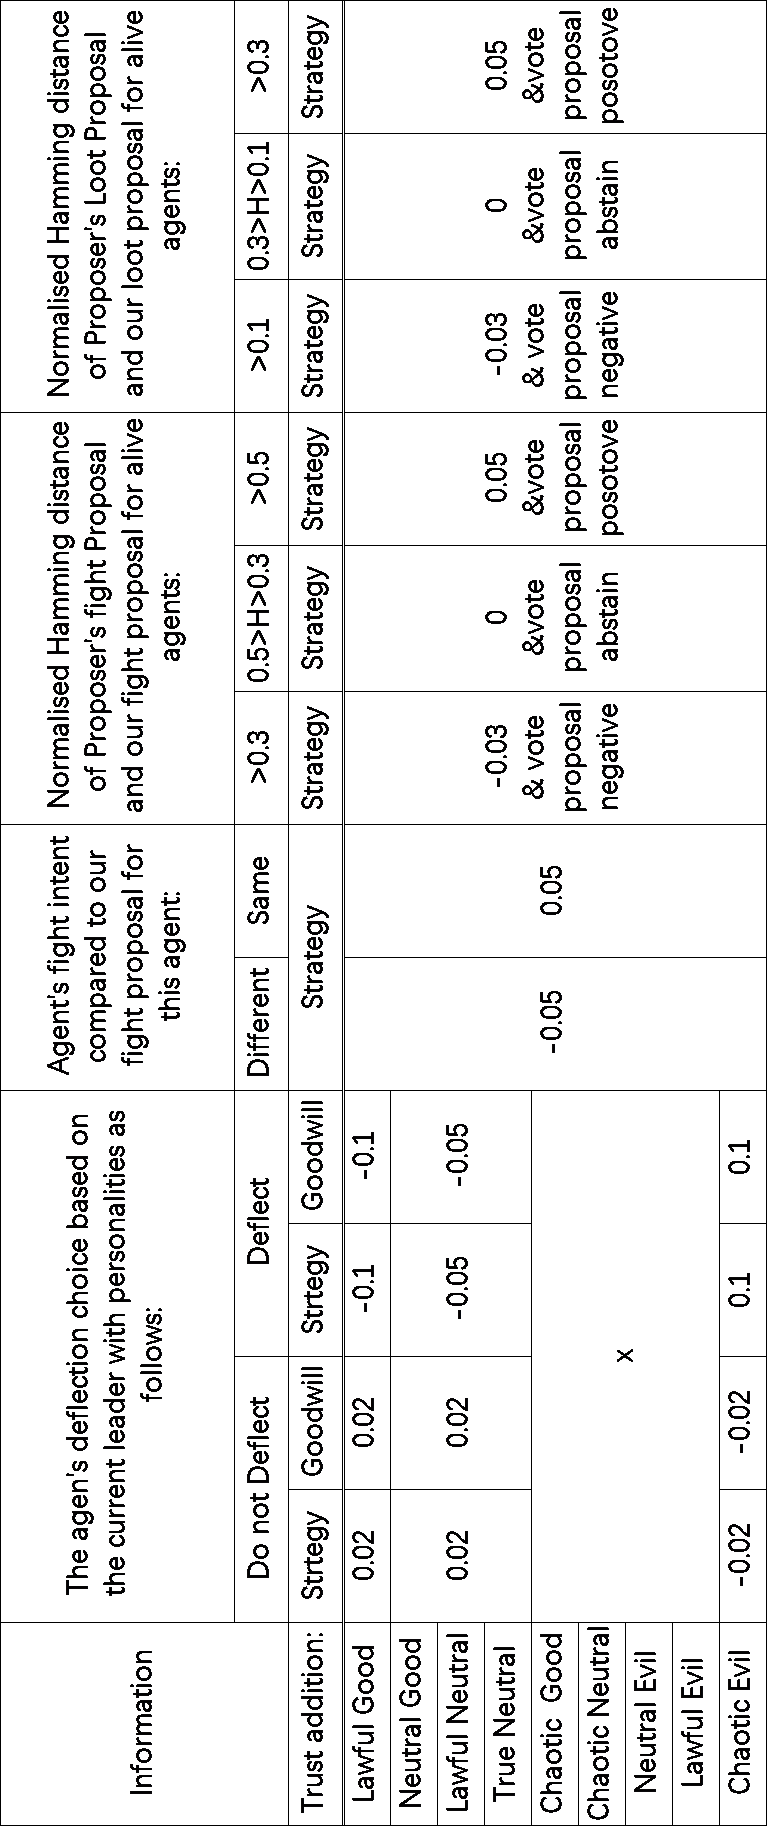
\includegraphics[scale=1]{008_team_5_agent_design/images/Information2Trusts.png}

\begin{SCfigure}[0.5][h]
    \caption{Details of updating trusts regarding different information that can be collected.}
    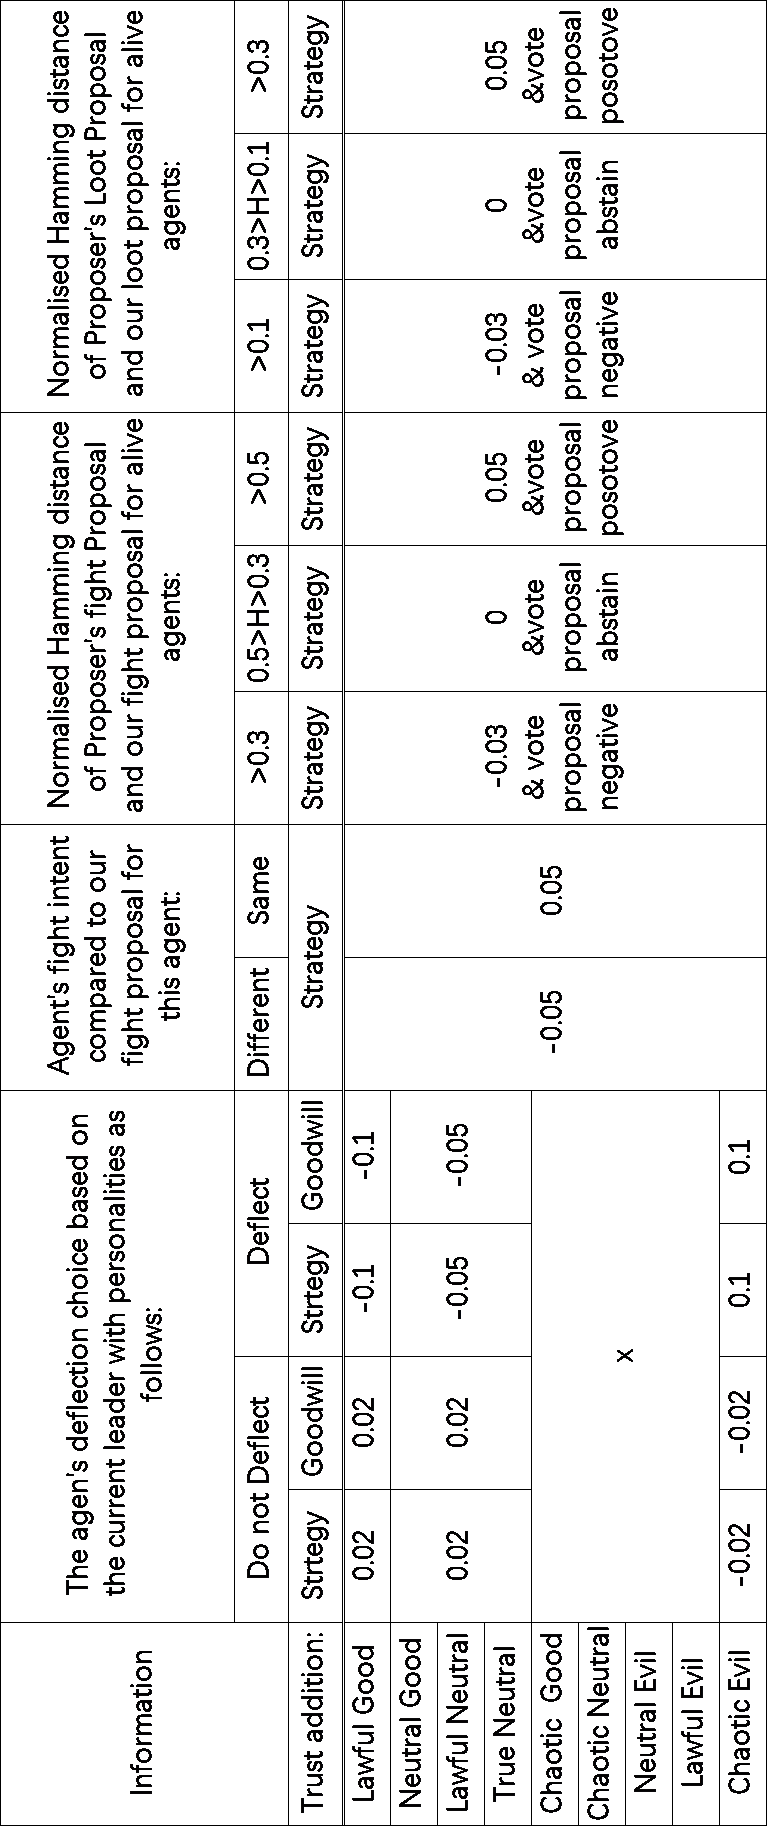
\includegraphics[width=0.63\textwidth]{008_team_5_agent_design/images/Information2Trusts.png}
    \label{fig:Information2Trusts}
\end{SCfigure}
\clearpage

\begin{figure}
    \centering
    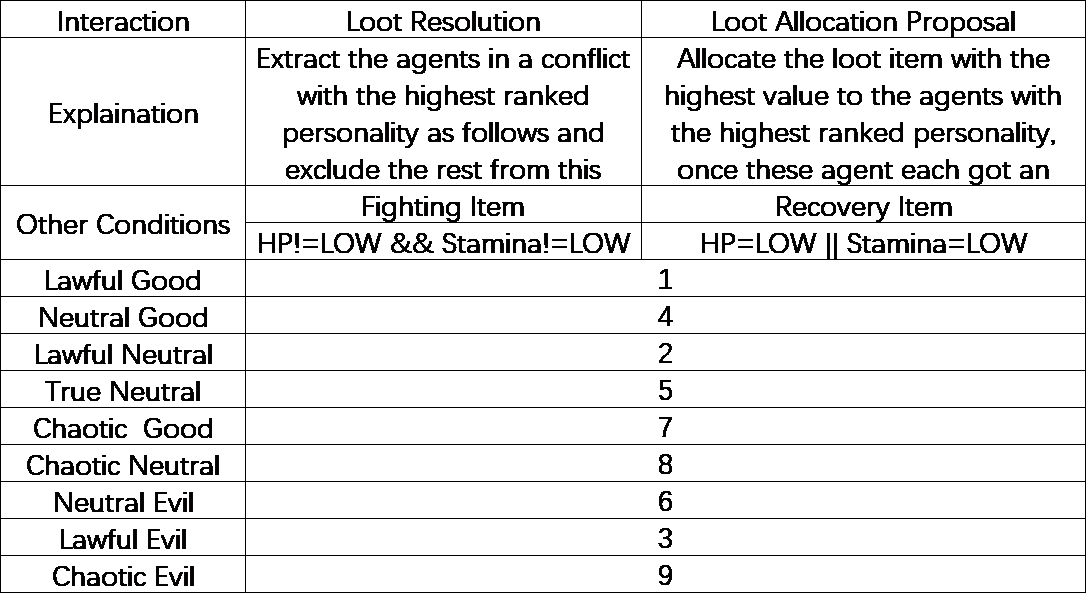
\includegraphics[scale=1]{008_team_5_agent_design/images/Interaction.png}
    \caption{Other agents' personality impact on our agent's interaction behaviour}
    \label{fig:my_label}
\end{figure}


\section{Election}



\section{Leadership Logic}
\subsection{Fight}
\subsection{Loot Allocation}
\subsection{Manifesto}



\section{Fight Logic}



\section{Trading Logic}



\section{Experiment}
